\documentclass[10pt]{article}
\usepackage[margin=1.6cm, top=1.5cm, bottom=1.6cm]{geometry}
\usepackage[T1]{fontenc}
\usepackage[utf8]{inputenc}
\usepackage{times}
\usepackage{graphicx}
\usepackage{booktabs}
\usepackage{array}
\usepackage{caption}
\usepackage{titlesec}
\usepackage{enumitem}
\usepackage{hyperref}
\hypersetup{hidelinks, colorlinks=false}

\setlength{\parindent}{0pt}
\setlength{\parskip}{4pt}
\titleformat{\section}{\bfseries\normalsize}{\thesection.}{0.4em}{}
\titleformat{\subsection}{\bfseries\small}{\thesubsection}{0.4em}{}
\titlespacing*{\section}{0pt}{9pt}{3pt}
\titlespacing*{\subsection}{0pt}{6pt}{2pt}
\captionsetup{font=small, labelfont=bf, skip=3pt}
\renewcommand{\arraystretch}{1.15}
\newcommand{\tablab}{\small}

\begin{document}

% ── Encabezado ──────────────────────────────────────────────────
\begin{center}
{\LARGE\bfseries Lab 1 $\cdot$ Modelado OLTP $\rightarrow$ OLAP}\\[4pt]
{\large PayTrack Colombia: esquema estrella, carga ELT y comparación de rendimiento}\\[6pt]
{\small SI7006 Almacenamiento y Procesamiento de Grandes Datos $\cdot$ Maestría en Ingeniería de Datos, EAFIT\\[2pt]
Integrantes: Samuel Gutiérrez Jaramillo $\cdot$ Alejandro Rendón Correa}
\end{center}
\vspace{2pt}
\hrule
\vspace{4pt}

% ── 1. Diagnóstico OLTP ────────────────────────────────────────
\section{Diagnóstico del esquema OLTP (Parte A)}

Se ejecutaron las tres consultas analíticas de \texttt{oltp\_problems.sql} con \texttt{EXPLAIN ANALYZE} sobre 50.000 y 500.000 transacciones. Resumen de los planes:

\vspace{2pt}
{\small
\begin{center}
\begin{tabular}{@{}p{1.1cm}p{5.6cm}p{5.6cm}r@{\hspace{8pt}}r@{}}
\toprule
\textbf{Consulta} & \textbf{Plan dominante (50K)} & \textbf{Plan dominante (500K)} & \textbf{$t_{50K}$} & \textbf{$t_{500K}$} \\
\midrule
Q1 & Bitmap Index Scan (\texttt{created\_at}) $\rightarrow$ Hash Join con \texttt{merchants} $\rightarrow$ HashAggregate & Parallel Seq Scan $\rightarrow$ Hash Join (2 workers) & 34{,}3 ms & 46{,}6 ms \\
Q2 & Seq Scan de \texttt{transactions} (sin filtro) $\rightarrow$ Hash Join con \texttt{customers} & Parallel Seq Scan (tabla completa) $\rightarrow$ Hash Join & 13{,}9 ms & 57{,}7 ms \\
Q3 & Bitmap Index Scan (7 días) $\rightarrow$ Sort sobre \texttt{EXTRACT(...)} $\rightarrow$ GroupAggregate & Ídem; Sort de 3{,}3 MB sobre 41.424 filas & 4{,}6 ms & 51{,}8 ms \\
\bottomrule
\end{tabular}
\end{center}
}

\textbf{Q1 (monto por categoría).} El filtro de fecha sí aprovecha \texttt{idx\_txn\_created\_at}, pero \texttt{category} vive en \texttt{merchants}: la 3FN obliga a recomponer mediante un \emph{join} la información que el diseño deliberadamente separó. El filtro \texttt{status='approved'} no tiene índice propio y se evalúa fila por fila. A 182M de filas (500K/día $\times$ 365), el rango de 30 días cubriría $\sim$60M de filas unidas y agregadas en cada consulta; el tiempo crece con las filas procesadas, no con las 7 filas devueltas.

\textbf{Q2 (tasa de fraude por segmento).} Es el peor caso: no hay filtro de fecha, por lo que se escanea la tabla completa para devolver 3 filas (50.000 filas procesadas $\rightarrow$ 3 devueltas a 50K; 500.000 $\rightarrow$ 3 a 500K), y se une todo el histórico con \texttt{customers} solo para leer \texttt{segment}. Con 182M de filas el \emph{hash join} excedería la memoria y caería a disco temporal, con tiempos del orden de decenas de segundos.

\textbf{Q3 (día de la semana y hora).} El OLTP solo guarda un timestamp: \texttt{EXTRACT(DOW/HOUR)} debe calcularse fila por fila y \emph{ordenarse} antes de agrupar, y ninguna función calculada aprovecha un índice. Con 7 días $\times$ 500K = 3{,}5M de filas, el ordenamiento excedería la memoria y usaría disco. En resumen, el OLTP está diseñado para escribir, no para agregar: cada consulta repaga el mismo trabajo porque no conserva resultados agregados.

% ── 2. Diseño ──────────────────────────────────────────────────
\section{Diseño del esquema estrella (Parte B)}

\textbf{Proceso y grano.} El proceso modelado es el registro de transacciones de pago; el grano de \texttt{fact\_transactions} es \textbf{una fila por cada transacción procesada} (ni resumen diario, ni evento de fraude, ni movimiento bancario).

\textbf{Dimensiones.} Cinco dimensiones: \texttt{dim\_date}, \texttt{dim\_time} (calendario precalculado: día de la semana, fin de semana, período del día, sin \texttt{EXTRACT} en cada consulta), \texttt{dim\_customer}, \texttt{dim\_merchant} y \texttt{dim\_payment\_method}. Del OLTP \emph{no} pasan al DW los datos personales del cliente (\texttt{name}, \texttt{email}, PII) ni el \texttt{method\_id} serial (llave técnica inestable). Como atributo conformado se agrega \texttt{method\_type} (tarjeta / billetera digital / transferencia bancaria), inexistente en el OLTP.

\textbf{Medidas.} \texttt{amount\_cop}, \texttt{is\_fraud} e \texttt{is\_approved} son \textbf{aditivas} (sumables en cualquier dimensión); \texttt{fraud\_risk\_score} es \textbf{no aditiva} (promediable, no sumable) y puede ser nulo: no toda transacción tiene evento de fraude.

\textbf{Surrogate keys.} Se usan llaves sustitutas numéricas en lugar de las llaves del OLTP porque: (1) permiten el versionamiento SCD2, donde un cliente ocupa varias filas; (2) desacoplan el DW de los sistemas operativos; (3) reducen el tamaño en disco y aceleran los \emph{join} (INTEGER vs.\ VARCHAR).

\textbf{SCD Tipo 2 en cliente.} El cliente puede cambiar de ciudad o de segmento. Si se sobrescribe el valor, todas las transacciones pasadas ``cambiarían de segmento'' retroactivamente y la tasa de fraude histórica quedaría distorsionada. SCD2 conserva cada versión con \texttt{valid\_from}/\texttt{valid\_to} y marca la vigente con \texttt{is\_current}; por eso la PK no puede ser \texttt{customer\_id} (sería no única entre versiones) sino la surrogate key \texttt{customer\_key}. En la carga inicial: \texttt{valid\_from} = creación del cliente, \texttt{valid\_to} = \texttt{'infinity'}, \texttt{is\_current} = \texttt{TRUE}. El comercio es SCD1 (atributos estables); el método de pago conserva \texttt{method\_name} como llave natural.

\textbf{Índices de la hechos.} \texttt{date\_key} (Q1/Q3), \texttt{merchant\_key} (Q1), \texttt{customer\_key} (Q2) y un índice parcial \texttt{merchant\_key WHERE is\_fraud} para análisis de solo fraude; su efecto real se midió con \texttt{EXPLAIN ANALYZE} (Sección~4).

\begin{figure}[h]
\centering
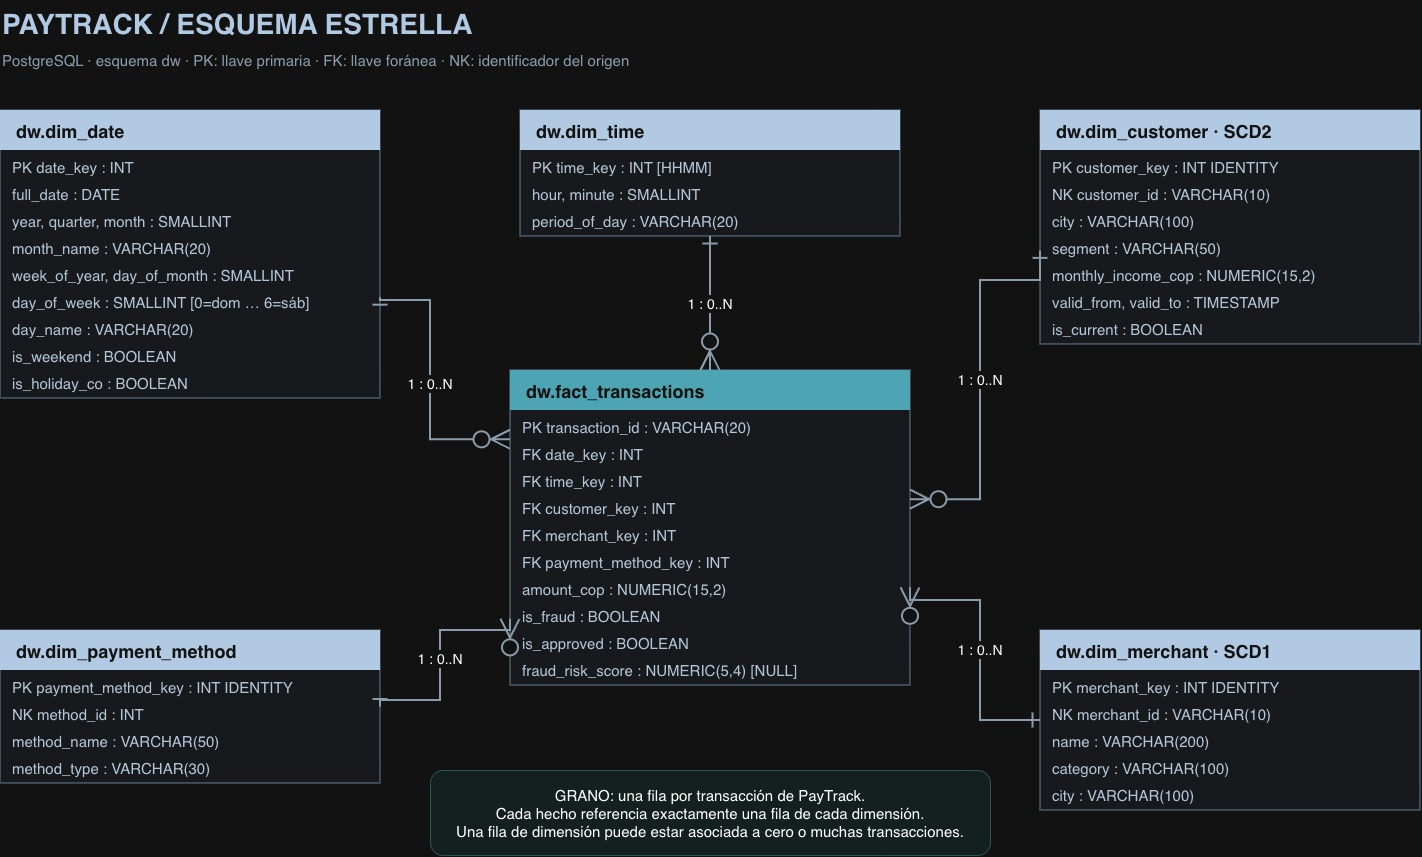
\includegraphics[width=0.72\textwidth]{figuras/diagrama.jpeg}
\caption{Esquema estrella PayTrack: 5 dimensiones, tabla de hechos y SCD2 de cliente.}
\end{figure}

% ── 3. Carga ELT ───────────────────────────────────────────────
\section{Carga ELT y validación (Parte C)}

El proceso ELT (4 \texttt{INSERT\,\ldots\,SELECT} de \texttt{oltp.*} a \texttt{dw.*}) traduce cada llave natural a su surrogate key; para el cliente une la transacción con la versión vigente en su fecha (\texttt{created\_at} entre \texttt{valid\_from} y \texttt{valid\_to}), deriva \texttt{date\_key} (AAAAMMDD), \texttt{time\_key} (HHMM) e \texttt{is\_approved} = (\texttt{status='approved'}), y trae \texttt{risk\_score} mediante \textbf{LEFT JOIN} con \texttt{fraud\_events} (solo $\sim$0{,}4\% de las transacciones tiene evento; un INNER JOIN habría descartado el resto). \texttt{verify()} valida conteos, montos, fraudes e integridad referencial.

\begin{figure}[h]
\centering
\begin{minipage}[t]{0.66\textwidth}
\centering
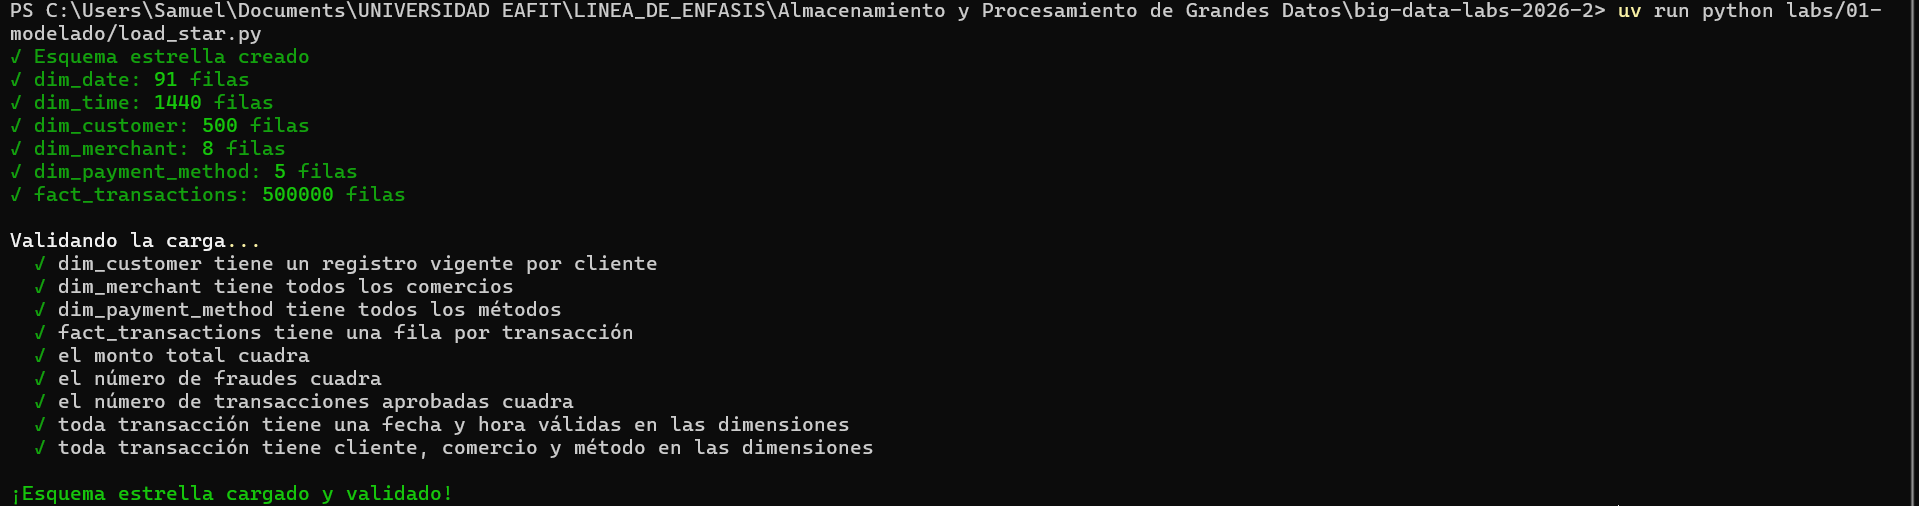
\includegraphics[width=\textwidth]{figuras/load_star_verde.png}
\caption{\texttt{load\_star.py}: 9 validaciones en verde (500K filas).}
\end{minipage}\hfill
\begin{minipage}[t]{0.32\textwidth}
\centering
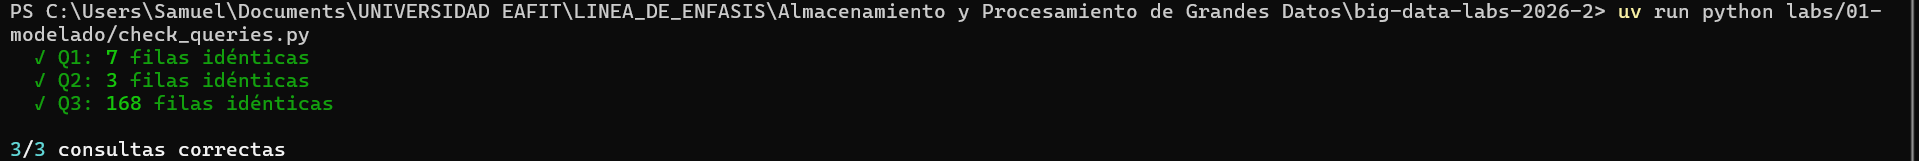
\includegraphics[width=\textwidth]{figuras/check_queries_3-3.png}
\caption{\texttt{check\_queries.py}: 3/3.}
\end{minipage}
\end{figure}

% ── 4. Consultas OLAP y rendimiento ────────────────────────────
\section{Consultas OLAP, comparación de rendimiento e índices (Parte D)}

\textbf{Validación.} Las tres consultas se reescribieron usando únicamente \texttt{dw.*}, con las mismas columnas que la versión OLTP. El validador confirmó resultados idénticos: Q1 7 filas, Q2 3 filas, Q3 168 filas, verificado tanto a 50.000 como a 500.000 transacciones. En Q2 se agrupa por el segmento \emph{actual} del cliente: se lo identifica desde la versión asociada al hecho y se busca su versión vigente (\texttt{is\_current}), replicando el OLTP sin excluir transacciones históricas.

\textbf{Comparación de rendimiento.} Cinco repeticiones por modelo con estadísticas actualizadas y orden alternado; medianas:

\vspace{2pt}
{\small
\begin{center}
\begin{tabular}{@{}lcccc@{}}
\toprule
& \multicolumn{2}{c}{\textbf{50.000 transacciones}} & \multicolumn{2}{c}{\textbf{500.000 transacciones}} \\
\cmidrule(lr){2-3}\cmidrule(lr){4-5}
\textbf{Consulta} & \textbf{OLTP} & \textbf{OLAP} & \textbf{OLTP} & \textbf{OLAP} \\
\midrule
Q1 (monto por categoría)   & 10{,}1 ms & 14{,}6 ms & 46{,}6 ms & 54{,}3 ms \\
Q2 (tasa de fraude)        & 19{,}5 ms & 18{,}2 ms & 57{,}7 ms & 60{,}5 ms \\
Q3 (día/hora)              & 5{,}9 ms  & 9{,}6 ms  & 51{,}8 ms & 75{,}1 ms \\
\bottomrule
\end{tabular}
\end{center}
}

Extracto de los planes de Q1 con \texttt{EXPLAIN ANALYZE} a 500K (misma consulta en ambos modelos; los planes completos están en \texttt{labs/01-modelado/evidencias/}):

\vspace{2pt}
{\footnotesize
\begin{minipage}[t]{0.485\textwidth}
\begin{verbatim}
-- OLTP
Finalize GroupAggregate (actual time=42.4..46.2
  rows=7)  Group Key: m.category
  ->  Gather Merge (2 workers)
      ->  Hash Join (actual time=0.09..30.7
           rows=56358 loops=3)
          ->  Parallel Seq Scan on transactions t
               Filter: (status='approved') AND
                 (created_at >= CURRENT_DATE-30)
               Rows Removed by Filter: 110309
Execution Time: 46.589 ms
\end{verbatim}
\end{minipage}\hfill
\begin{minipage}[t]{0.485\textwidth}
\begin{verbatim}
-- OLAP
Finalize GroupAggregate (actual time=47.9..54.0
  rows=7)  Group Key: m.category
  ->  Gather Merge (2 workers)
      ->  Hash Join (f.merchant_key =
           m.merchant_key) rows=56358
          ->  Hash Join (f.date_key = d.date_key)
               ->  Parallel Seq Scan on
                    fact_transactions f
                    Filter: is_approved
Execution Time: 54.303 ms
\end{verbatim}
\end{minipage}
}

En Q1 y Q3 a 50K, el OLTP usó el índice de fecha (17.006 y 4.284 filas del período); el OLAP recorrió los 50.000 hechos y filtró mediante \emph{join}: el planificador prefirió un \emph{sequential scan} sobre \texttt{fact\_transactions} en vez de \texttt{idx\_fact\_date}, decisión razonable en tablas pequeñas. A 500K, Postgres activó dos trabajadores paralelos y ambos modelos escalaron de manera sublineal (10$\times$ datos $\rightarrow$ $\sim$5$\times$ tiempo), manteniéndose las diferencias en el mismo rango de magnitud.

\textbf{Índices.} Retirarlos individualmente produjo variaciones inferiores al 1,6\%: ninguno apareció en los planes iniciales, porque con tablas de este tamaño recorrer la tabla completa resulta más barato que el acceso por índice. El índice parcial de fraude no cubre por sí solo Q2, pues la tasa también requiere contar las transacciones no fraudulentas. Análogamente, \texttt{is\_approved} conserva el 99,87\% de las filas (Q2 necesita todas), lo que explica la preferencia por el \emph{sequential scan}.

\textbf{Conclusión.} El esquema estrella produce resultados correctos, validados uno a uno contra el OLTP a ambas escalas. En este experimento el acceso por índice de fecha favoreció al OLTP en Q1 y Q3, y Q2 fue ligeramente más rápida en OLAP a 50K (equivalente a 500K); como advierte el propio README, con estas escalas las diferencias son pequeñas. El valor del modelo dimensional no se limita al tiempo de respuesta: garantiza acceso directo a los atributos de agrupación (categoría, segmento, día, hora) sin recalcularlos ni unir tablas normalizadas, y conforme el volumen crece hacia las 500K transacciones diarias del caso de uso, las agregaciones sobre dimensiones precalculadas escalan de manera más predecible que los \emph{join} repetidos sobre un esquema OLTP.

\end{document}
